\chapter{Appendix}

%\section{Contents of the accompanying cloud storage}

\section{Additional plots for sharp borders experiment}\label{app:sharp}
In this section, we include the additional plots that were created for our first experiment with sharp region borders in the workload. \par 

\Cref{fig:app_exp1_query_dist} shows the query distributions that are created by our workload generation. \verb|fb| on the left presents the challenge that almost all keys are concentrated at the beginning of the dataset due to very large outliers. Therefore, our plot only shows a single bar representing most of the one million queries. For the wiki dataset on the right, we needed to increase our window size to $w = 20000$ to get our desired partitions; with $w = 10000$, our algorithm produced around 50 partitions.

\Cref{fig:app_exp1_poc_times} displays the average lookup times we obtained. Notice that the PGM index threw an exception during execution for the \verb|fb| dataset, which is why we do not have a data point there. We observe similar results to the three datasets presented in the main part of this work, with our index achieving around 250 ns as the average lookup time. We also note that the ART index can outperform our index on the \verb|wiki| dataset and achieves a comparable time to its performance on uniform dense data.


\begin{figure}
    \centering
    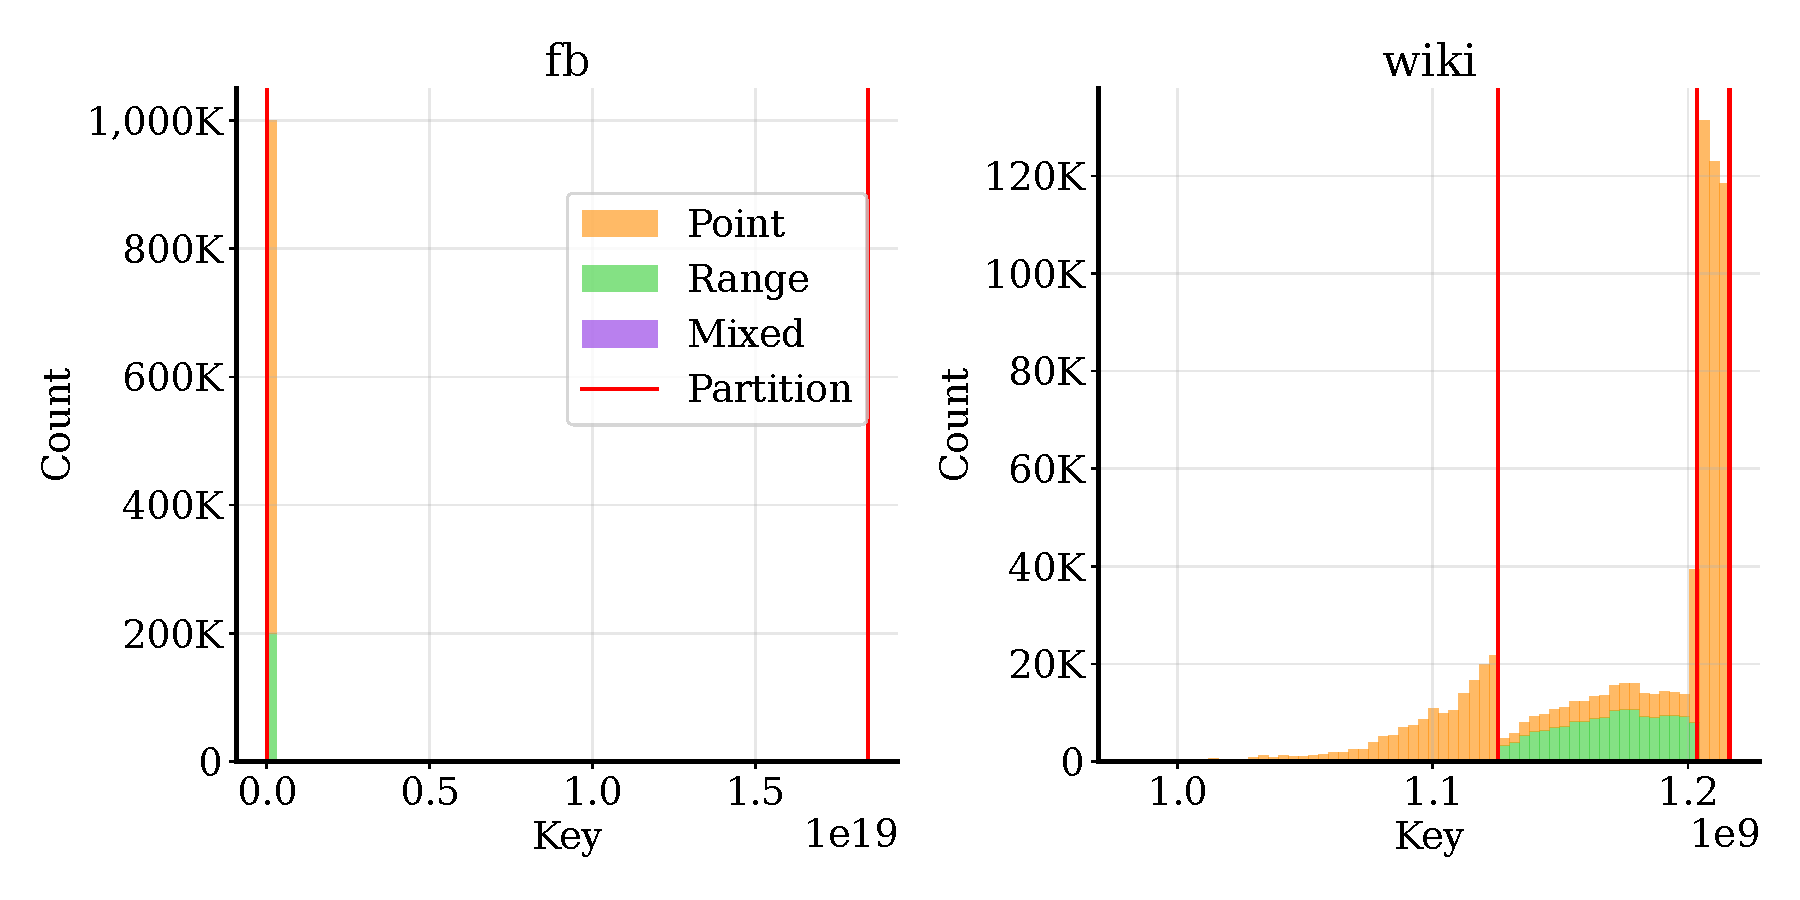
\includegraphics[width=\textwidth]{figures/app_exp1_query_dist.pdf}
    \caption[fb and wiki query distribution after sharp boundary sampling]{Query distribution for the workloads used in our first experiment. The queries were sampled on the real-world datasets fb and wiki with 200 million keys each.}
    \label{fig:app_exp1_query_dist}
\end{figure}

\begin{figure}
    \centering
    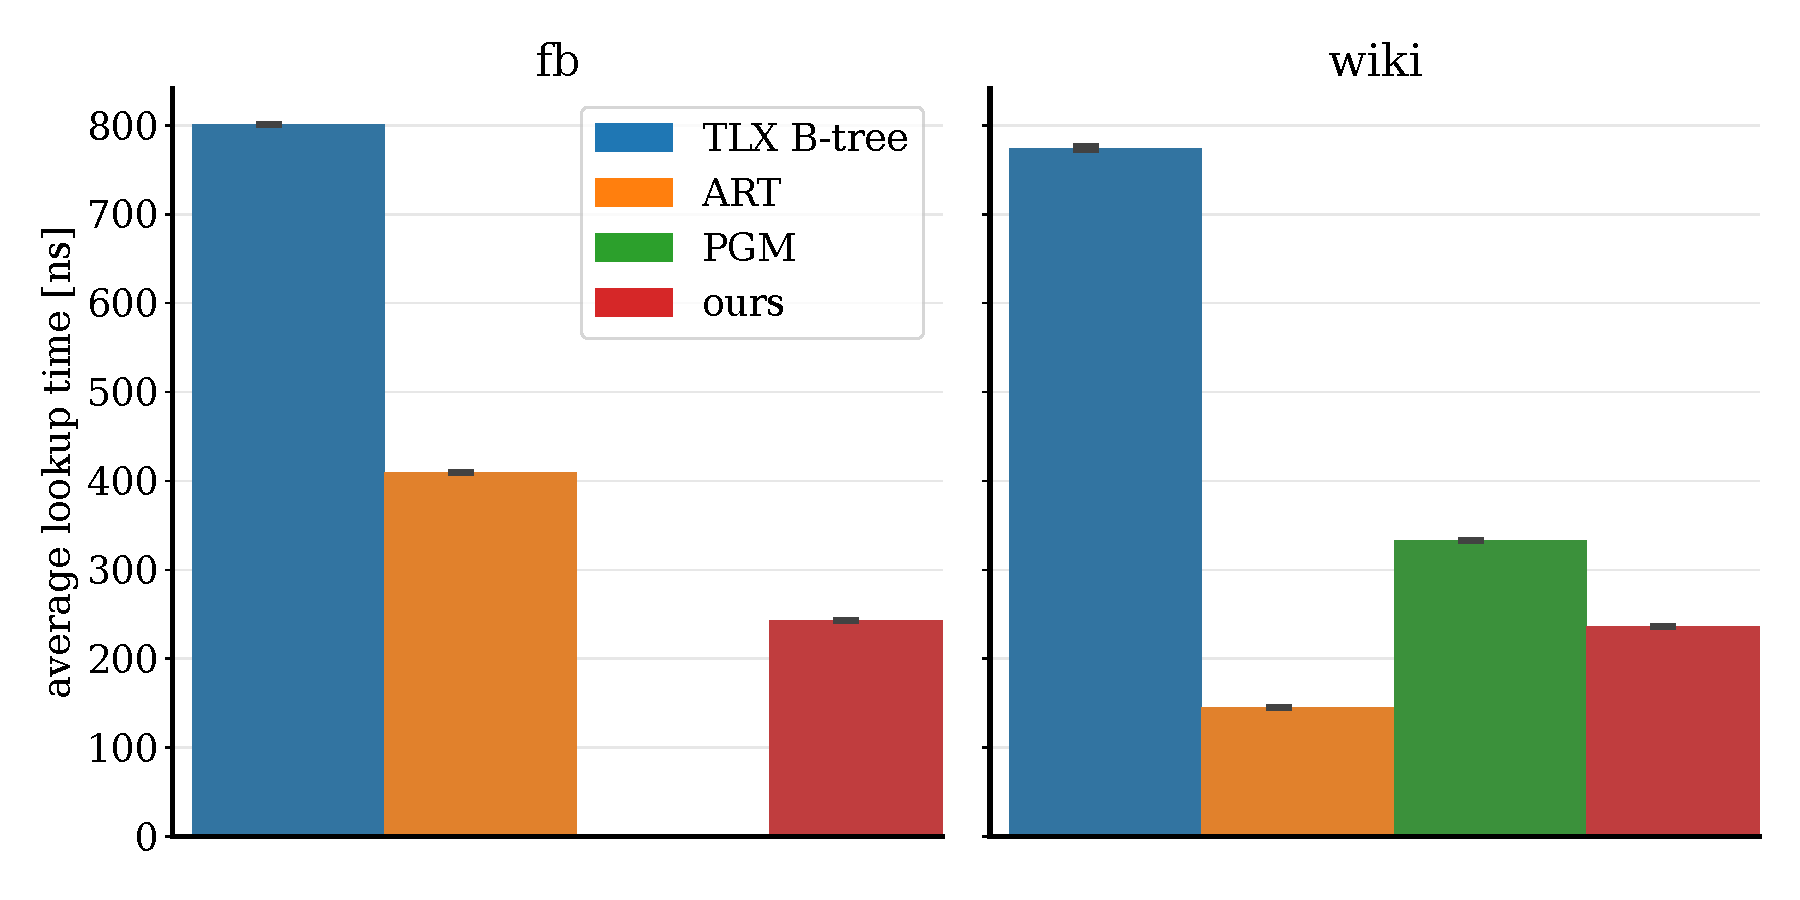
\includegraphics[width=\textwidth]{figures/app_exp1_poc_times.pdf}
    \caption[fb and wiki lookup performance after sharp boundary sampling]{Average query lookup time on the real-world datasets fb and wiki for our first experiment. The average is taken over one million queries.}
    \label{fig:app_exp1_poc_times}
\end{figure}

\clearpage
\section{Additional plots for skewed distributions experiment}\label{app:skew}
In this section, we include the additional plots that were created as part of the skewed workloads on a uniform dense and the osm dataset. The plots show sampling using a gamma distribution, which was very similar to the lognormal one we already used in the evaluation section. \par

\Cref{fig:app_exp2_query_dist} and \Cref{fig:app_exp2_poc_times} show the results. As we suspected, they are very similar to the ones we obtained from the lognormal sampling previously.

\begin{figure}[ht]
    \centering
    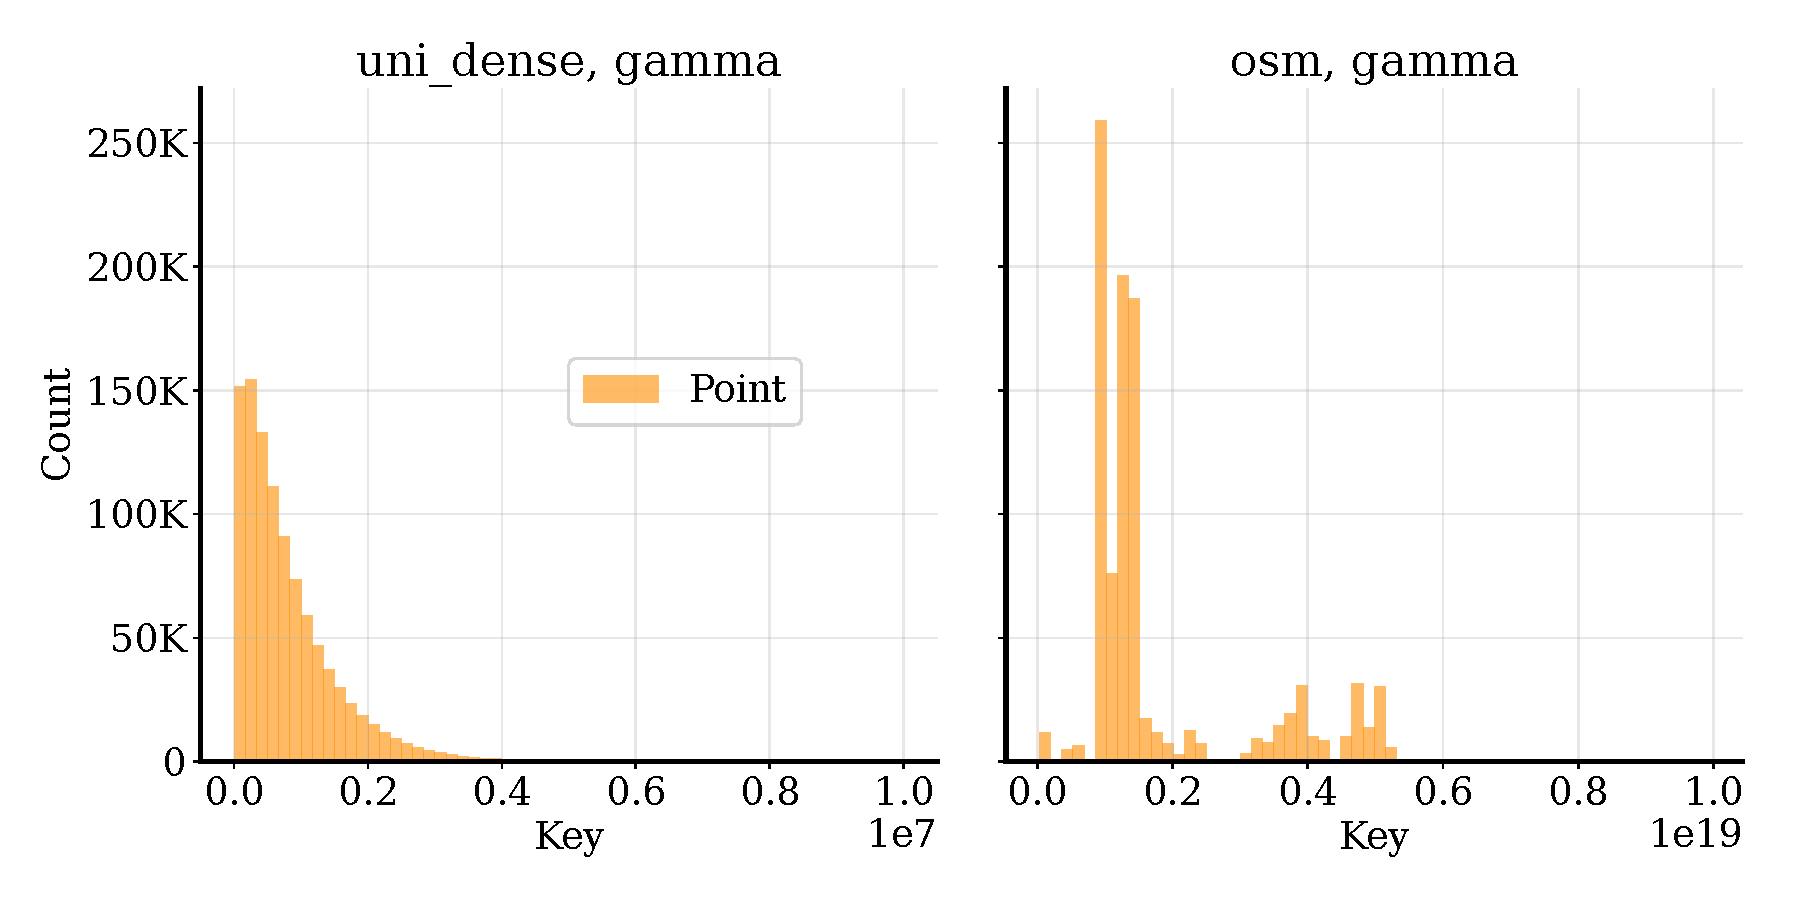
\includegraphics[width=0.75\textwidth]{figures/app_exp2_query_dist.pdf}
    \caption[uniform and osm query distributions after gamma sampling]{Query distribution for the gamma distributed workload. The queries were sampled on a uniform, dense dataset with 10 million keys, and the real-world dataset osm, downsampled to 10 million keys.}
    \label{fig:app_exp2_query_dist}
\end{figure}

\begin{figure}[ht]
    \centering
    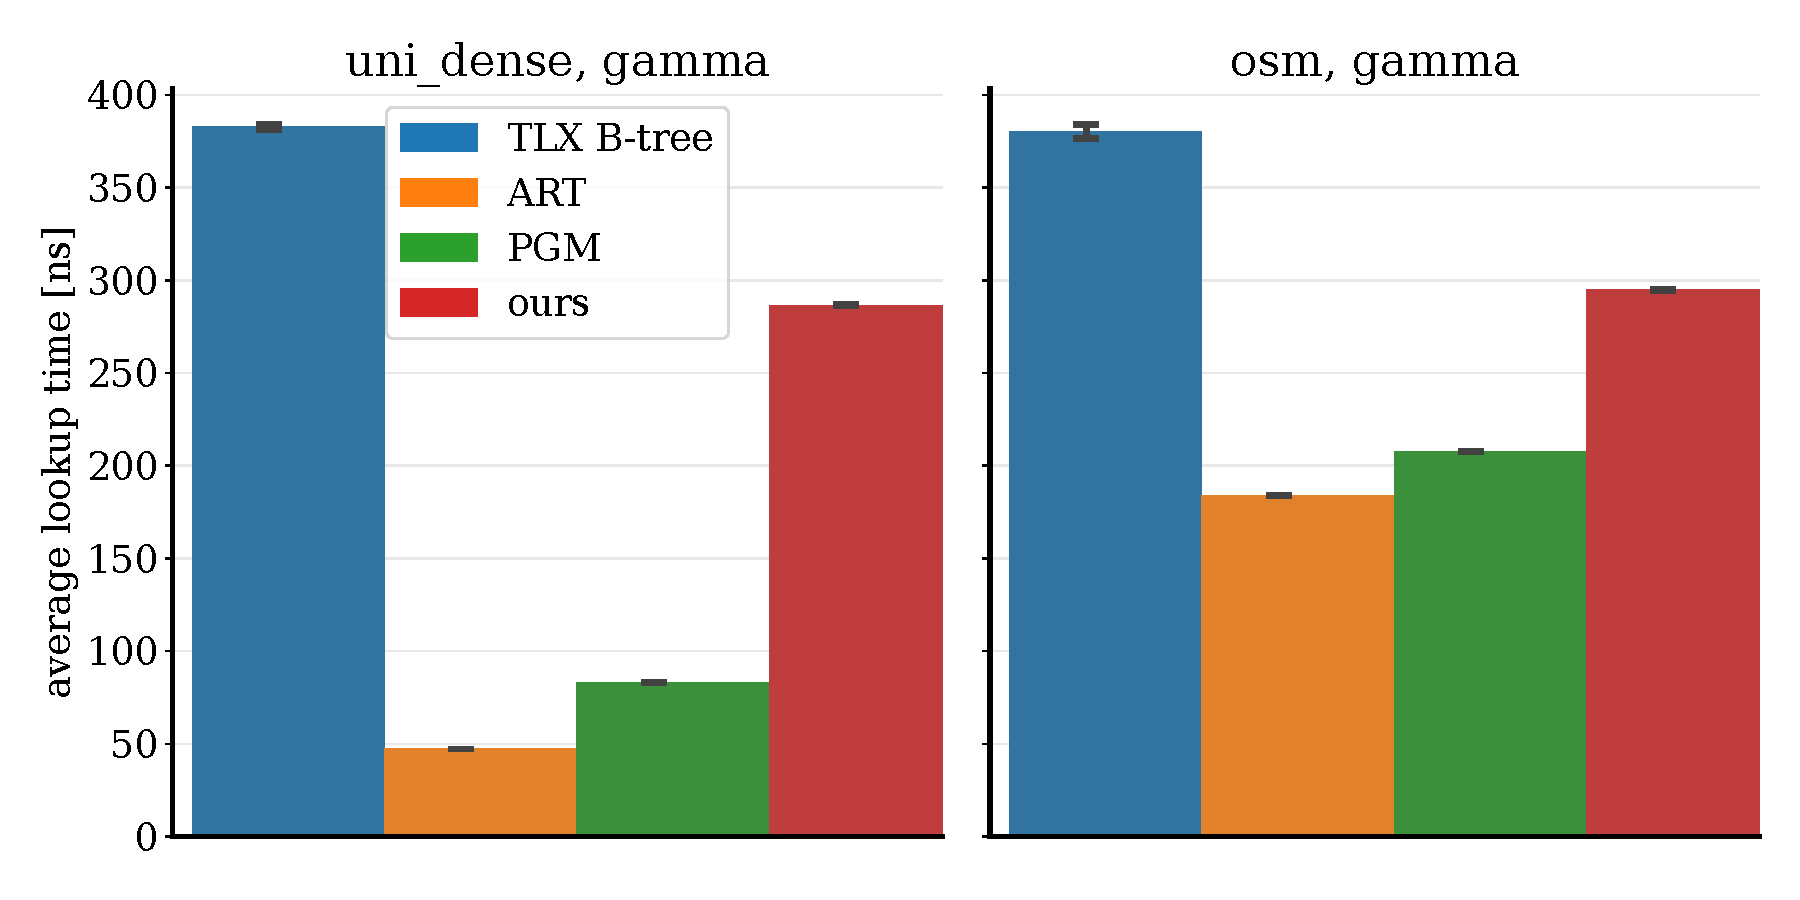
\includegraphics[width=0.75\textwidth]{figures/app_exp2_poc_times.pdf}
    \caption[uniform and osm lookup performance after gamma sampling]{Average query lookup time on a uniform, dense dataset with 10 million keys and the real-world dataset osm, downsampled to 10 million keys. The average is taken over one million queries.}
    \label{fig:app_exp2_poc_times}
\end{figure}


\section{Additional plots for index misses experiment}\label{app:misses}
This section includes the additional plots that show the workload distribution when we sample index-based and domain-based. Because the underlying \verb|osm| dataset is very sparse, the percentage of domain-based queries is very close to the percentage of index misses because the sampled queries are most likely not present in our data. \par

\Cref{fig:app_exp4_uni_query_dist}, \Cref{fig:app_exp4_normal_query_dist} and \Cref{fig:app_exp4_lognormal_query_dist} show the results. We observe that for an increasing amount of domain-based queries, the overall query distribution slowly transforms into a distribution that resembles sampling index-based on a uniform, dense dataset. This is simply since we indeed sample queries in the range of the minimal and maximal value in the data. The range is just the interval [min, max] and can therefore be seen as a uniform, dense dataset over which we sample.

\vfill
\begin{figure}[hb]
    \centering
    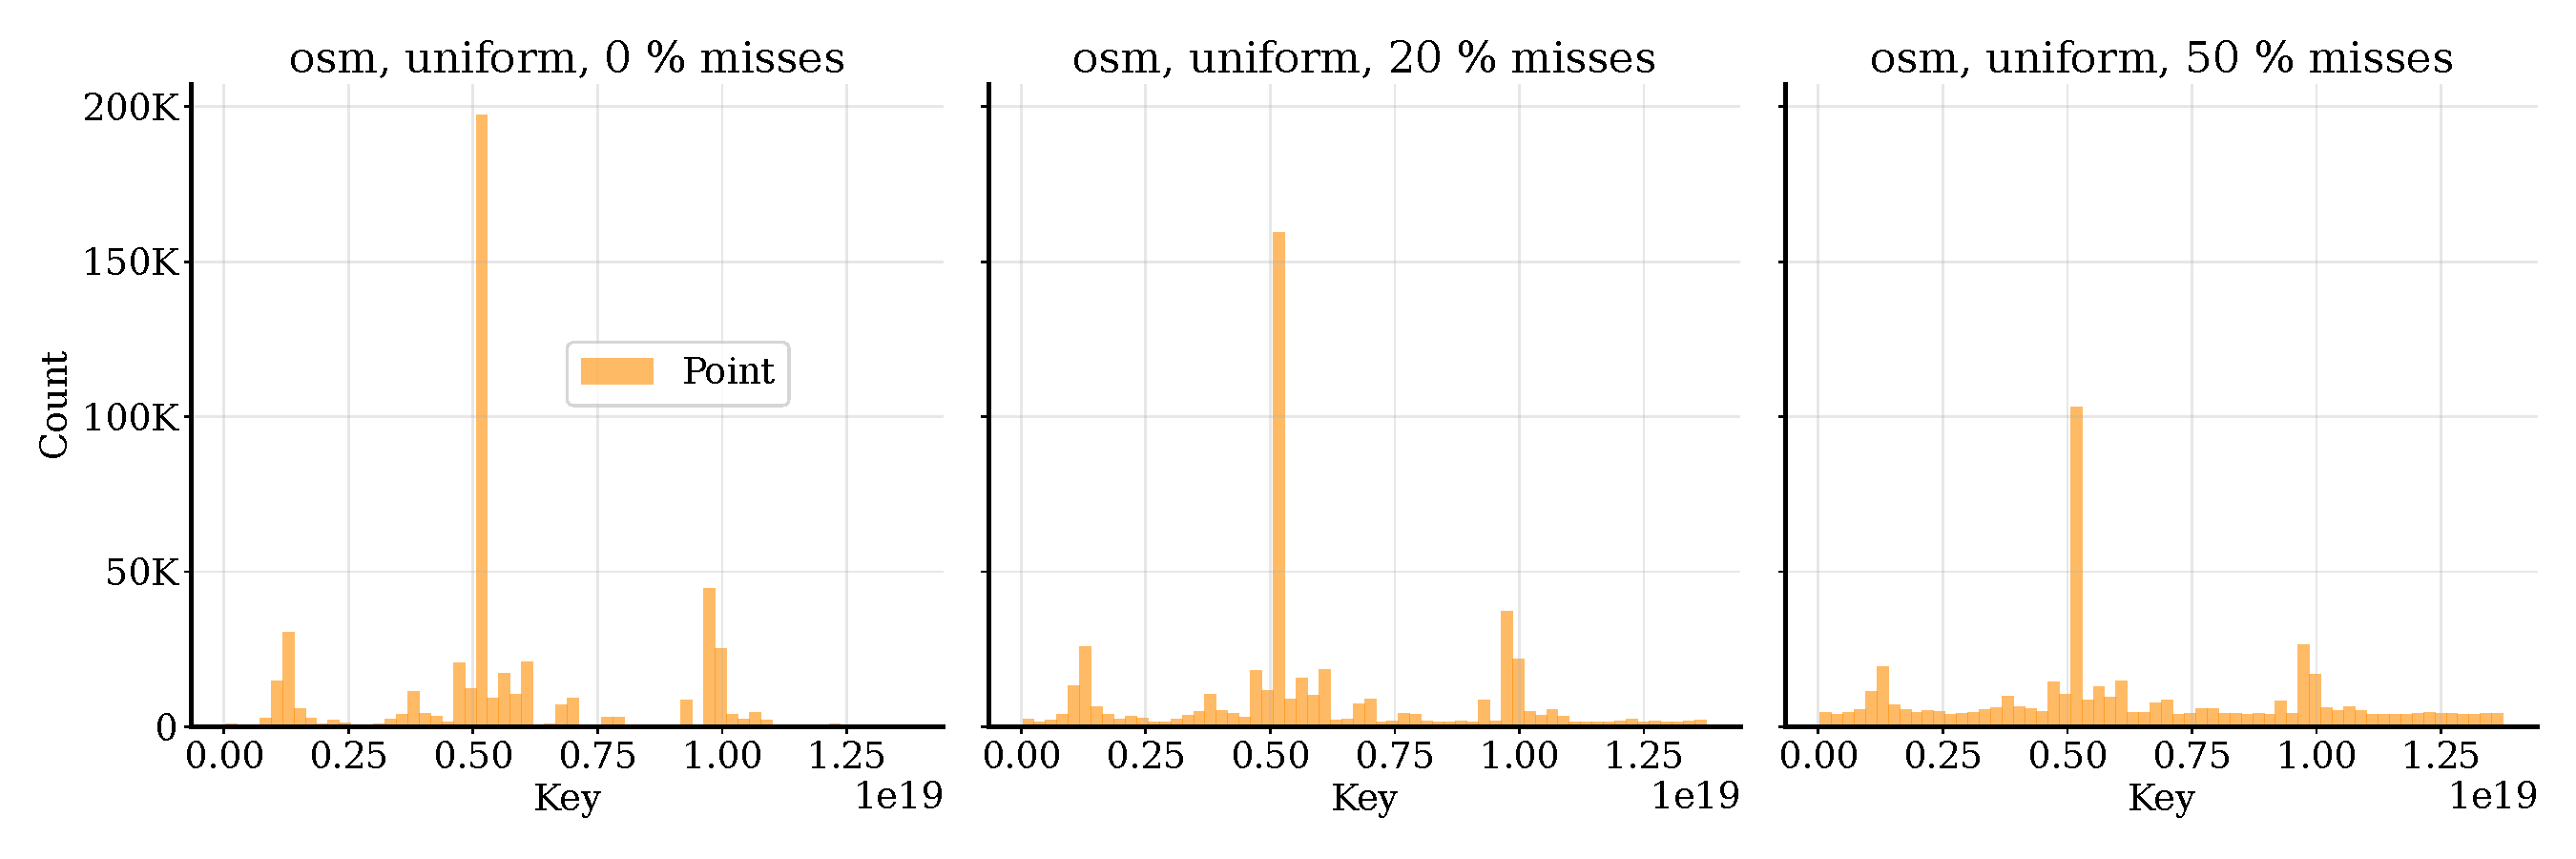
\includegraphics[width=\textwidth]{figures/app_exp4_uni_query_dist.pdf}
    \caption[osm query distribution after uniform sampling with index misses]{Query distribution for a uniform workload. The queries were sampled on the real-world dataset osm with 10 million keys. The first graph shows the distribution for no index misses, the second for 20 \% index misses and the third one for 50 \% index misses.}
    \label{fig:app_exp4_uni_query_dist}
\end{figure}
\vfill

\begin{figure}[ht]
    \centering
    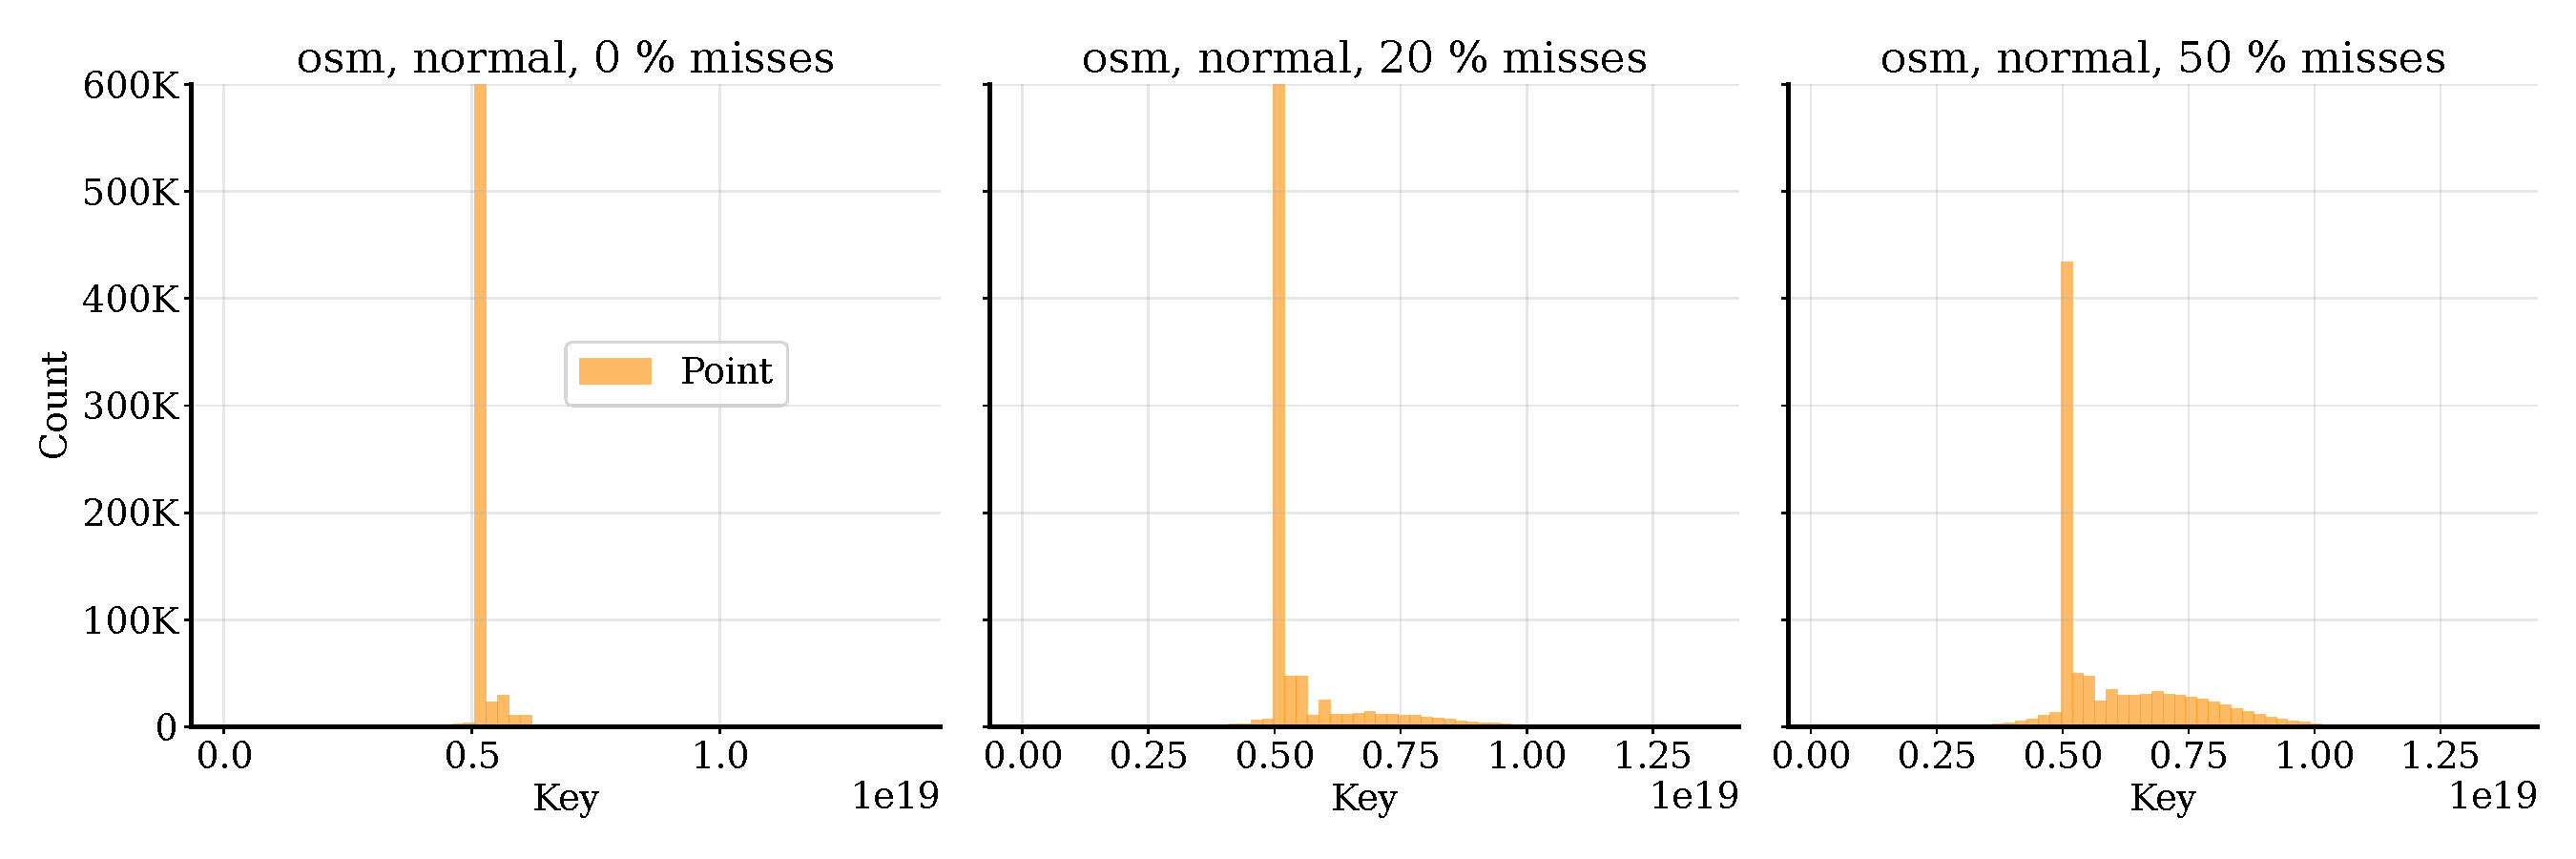
\includegraphics[width=\textwidth]{figures/app_exp4_normal_query_dist.pdf}
    \caption[osm query distribution after normal sampling with index misses]{Query distribution for a normal workload. The queries were sampled on the real-world dataset osm with 10 million keys. The first graph shows the distribution for no index misses, the second for 20 \% index misses and the third one for 50 \% index misses.}
    \label{fig:app_exp4_normal_query_dist}
\end{figure}

\begin{figure}[ht]
    \centering
    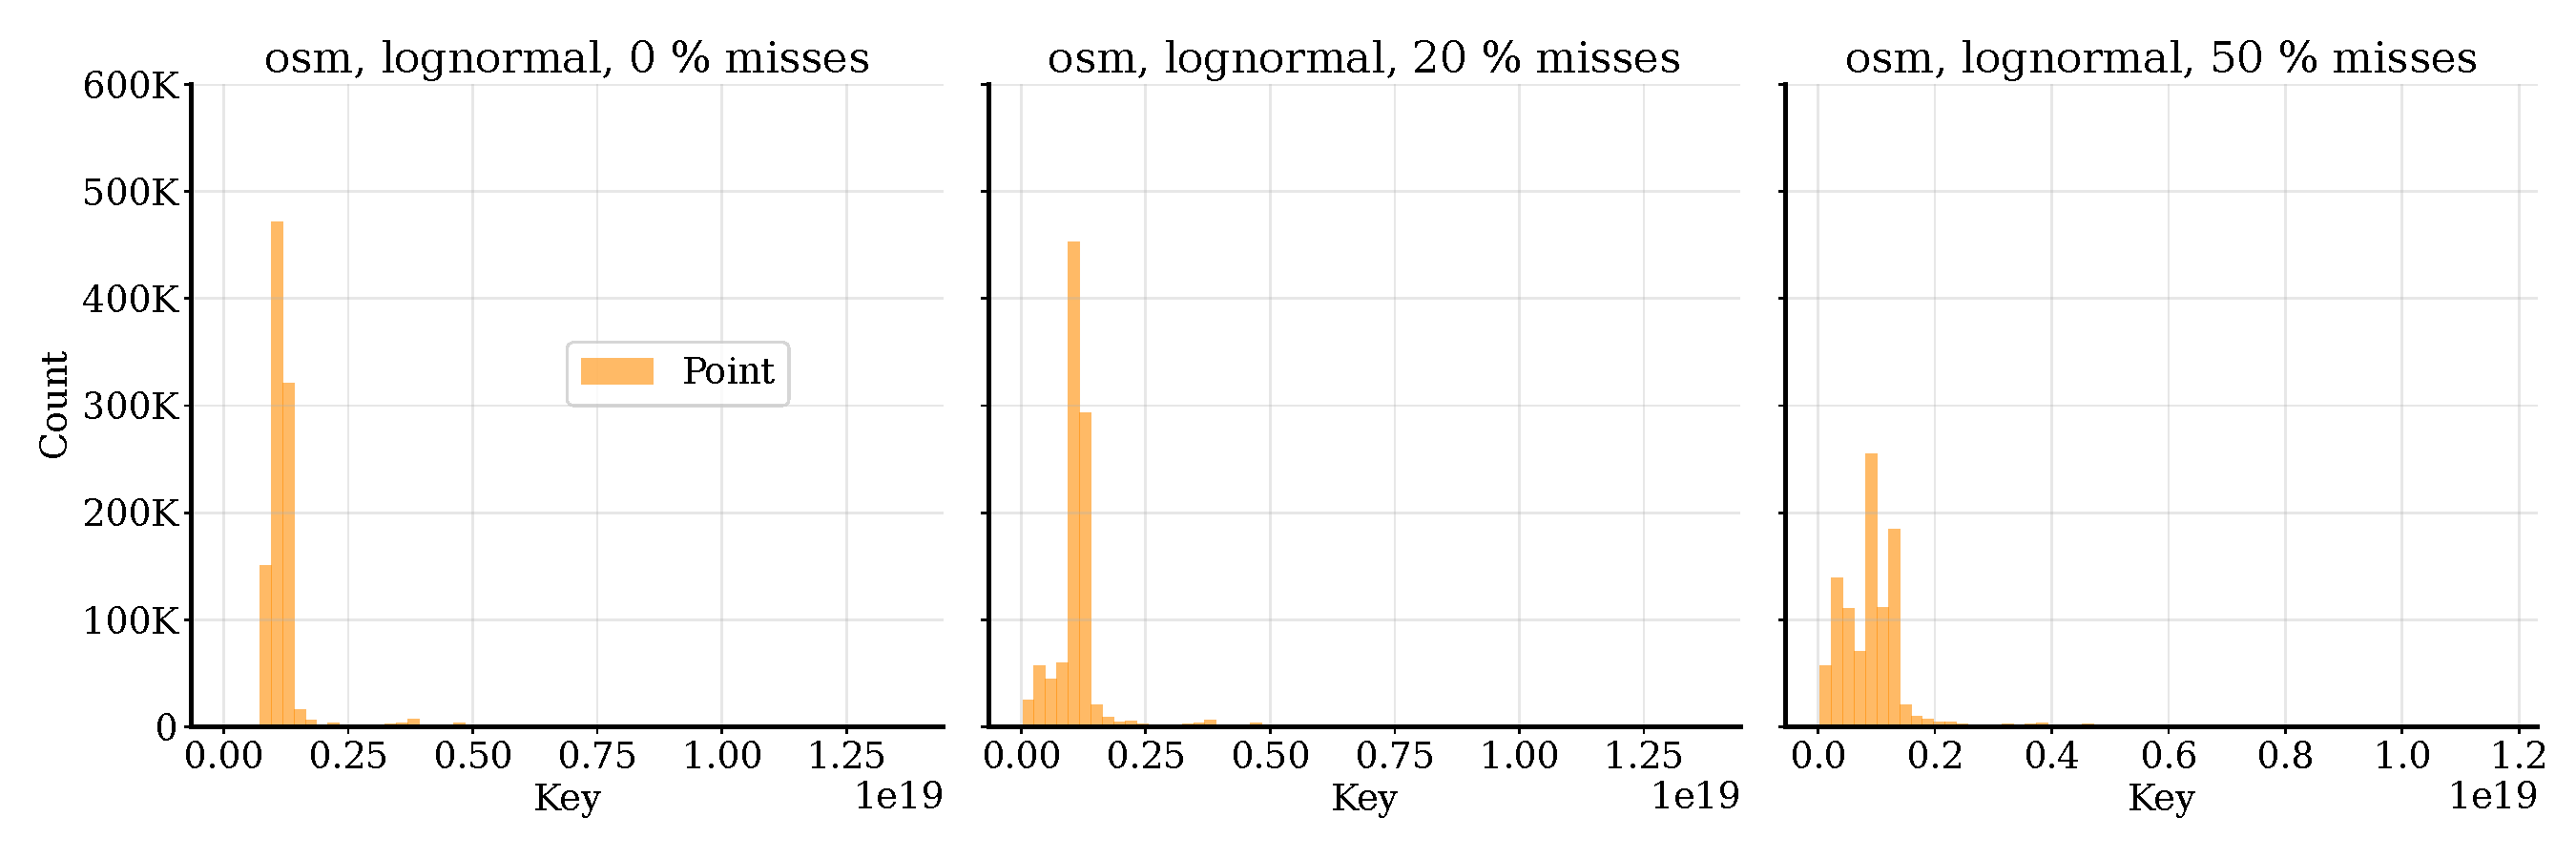
\includegraphics[width=\textwidth]{figures/app_exp4_lognormal_query_dist.pdf}
    \caption[osm query distribution after lognormal sampling with index misses]{Query distribution for a lognormal workload. The queries were sampled on the real-world dataset osm with 10 million keys. The first graph shows the distribution for no index misses, the second for 20 \% index misses and the third one for 50 \% index misses.}
    \label{fig:app_exp4_lognormal_query_dist}
\end{figure}